\chapter*{Appendix: Experimental material}
\begin{figure}[ht]
    \centering
    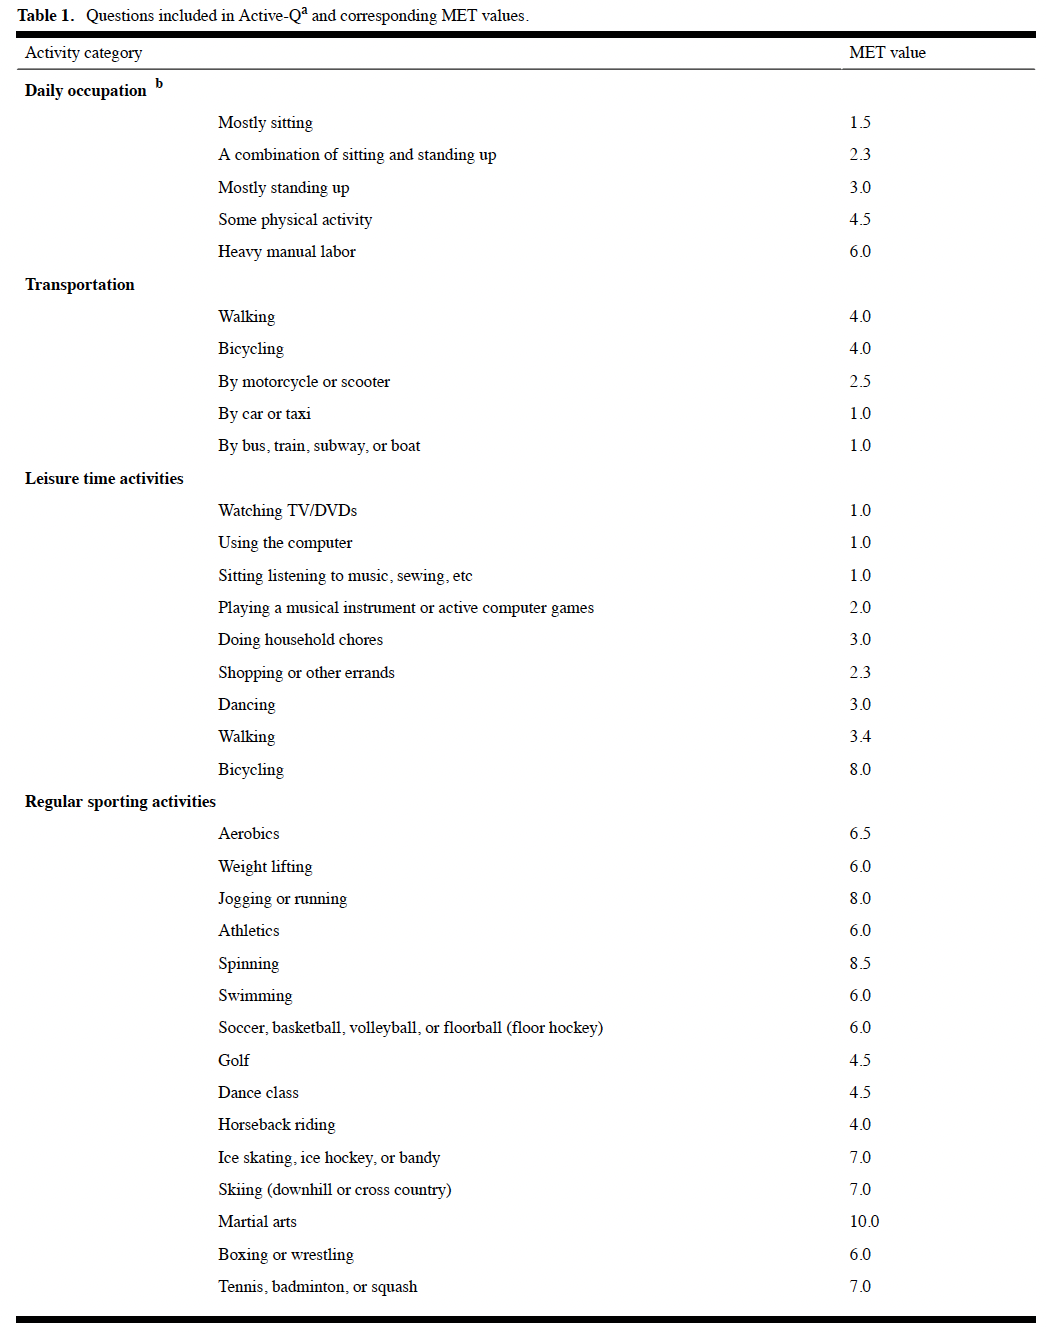
\includegraphics[width=0.8\textwidth]{appendix/met_values.png}
    \caption{MET value labels \parencite{Bonn_2012}}
    \label{fig: met_values}
\end{figure}
\begin{figure}[ht]
    \centering
    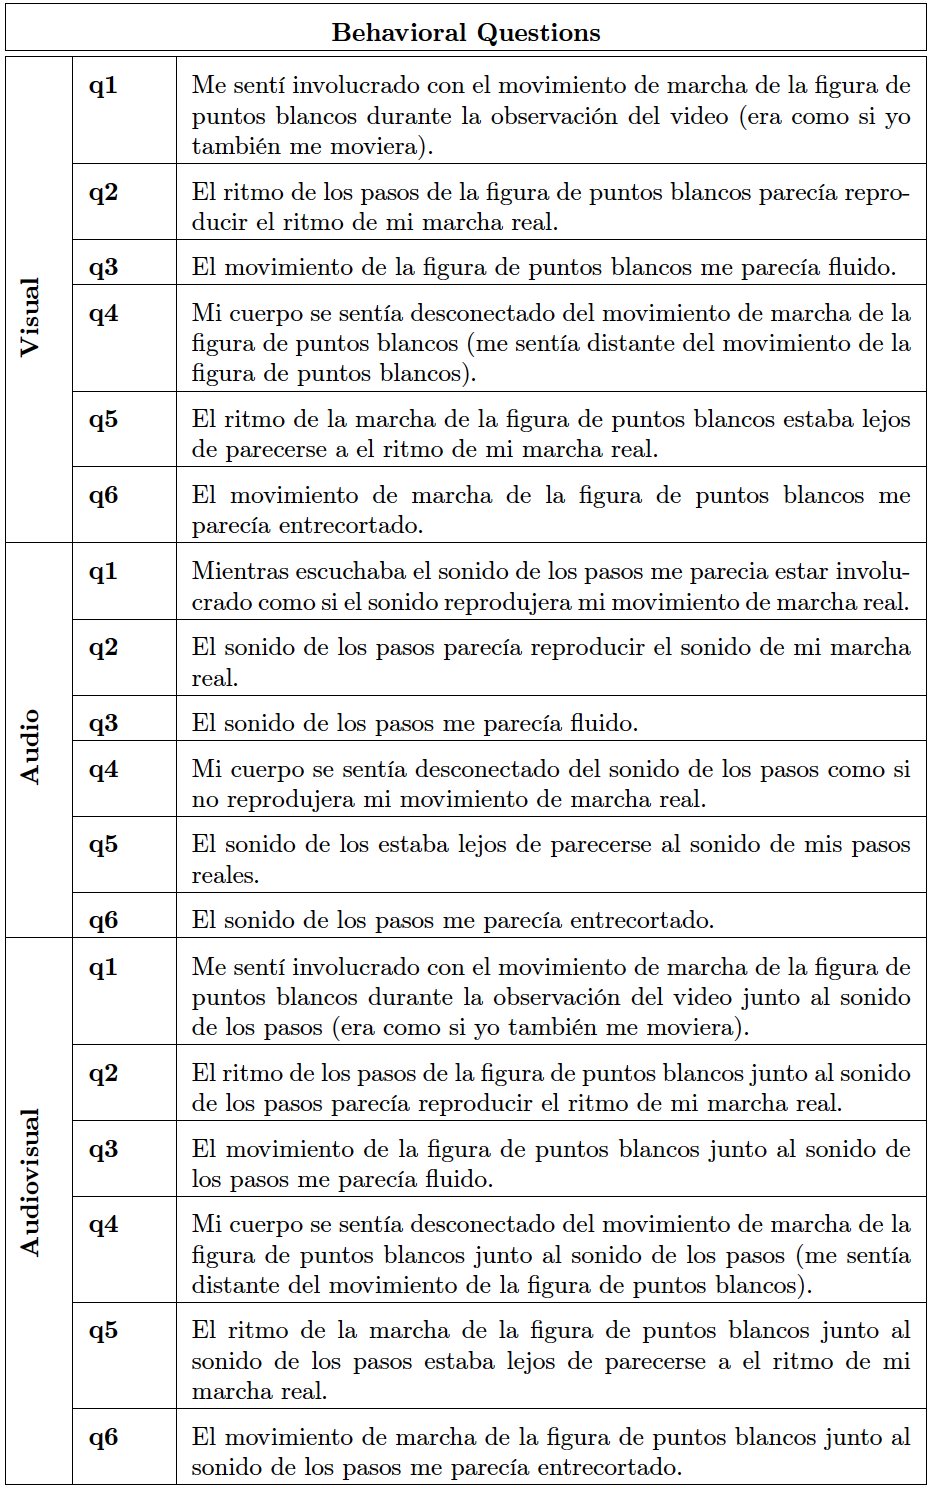
\includegraphics[width=0.70\textwidth]{appendix/questions.png}
    \caption{Behavioral questions translated in English from Spanish}
    \label{fig: Behavioral questions}
\end{figure}

\clearpage
\chapter*{Appendix: Statistical results tables}
\subsection*{Results related to behavioral questions}
\begin{figure}[H]
    \begin{subfigure}[b]{0.5\textwidth}
        \centering
        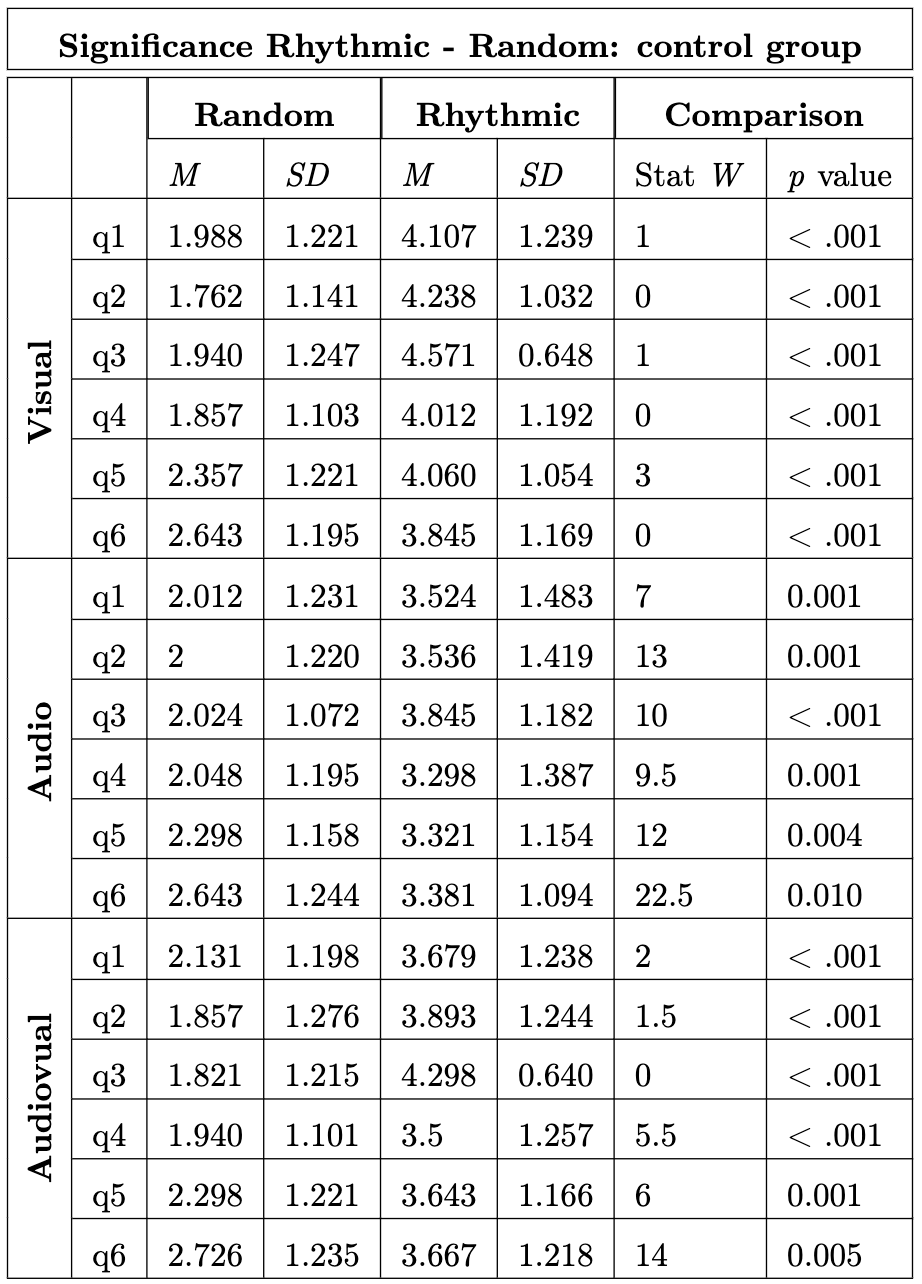
\includegraphics[width=\textwidth]{significance_tables/control_group.png}
        \caption{Significance of the results of behavioral questions in the control group, using Wilcoxon Signed-Rank Test (\textit{W}); \textit{M} = mean; \textit{SD} = standard deviation}
        \label{fig: significance_control_pop} 
    \end{subfigure}
    \begin{subfigure}[b]{0.5\textwidth}
        \centering
        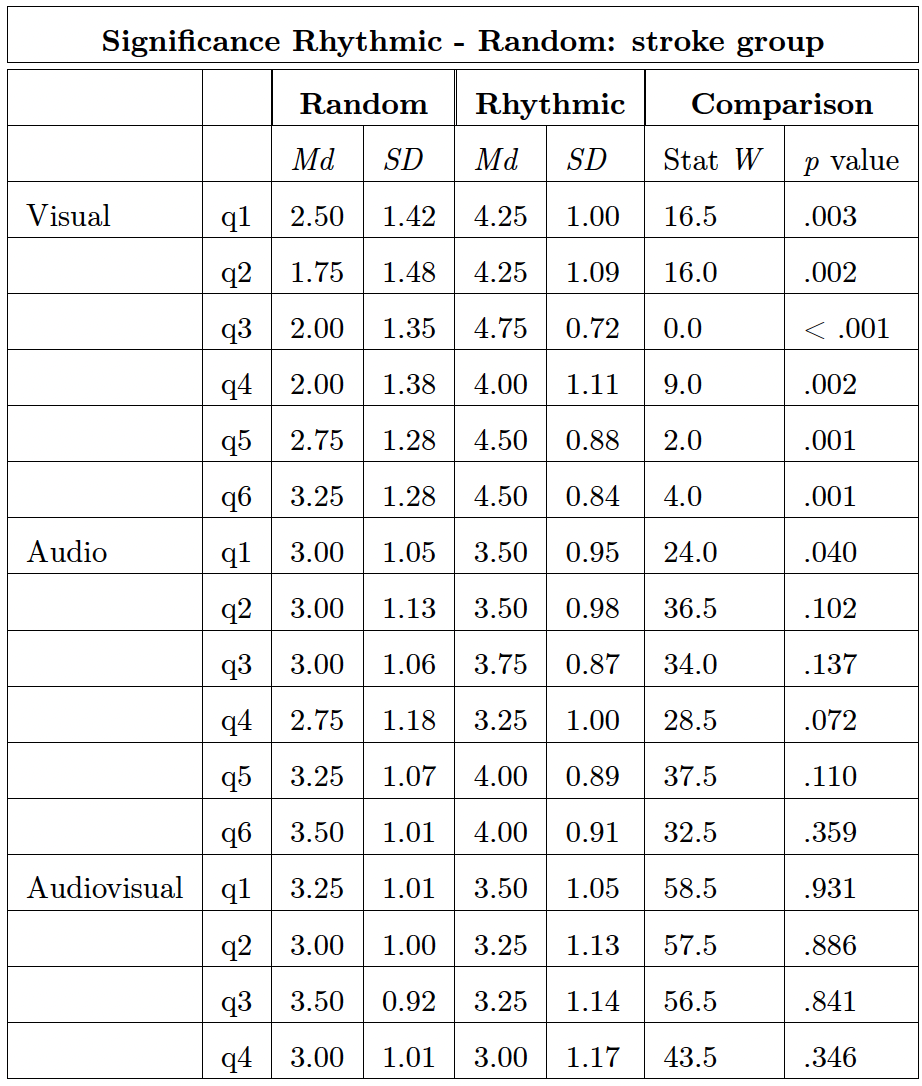
\includegraphics[width=\textwidth]{significance_tables/stroke_group.png}
        \caption{Significance of the results of behavioral questions in the stroke group, using Wilcoxon Signed-Rank Test (\textit{W}); \textit{M} = mean; \textit{SD} = standard deviation}
        \label{fig: significance_stroke_pop} 
    \end{subfigure}
\end{figure} 

\begin{figure}[H]
    \centering
    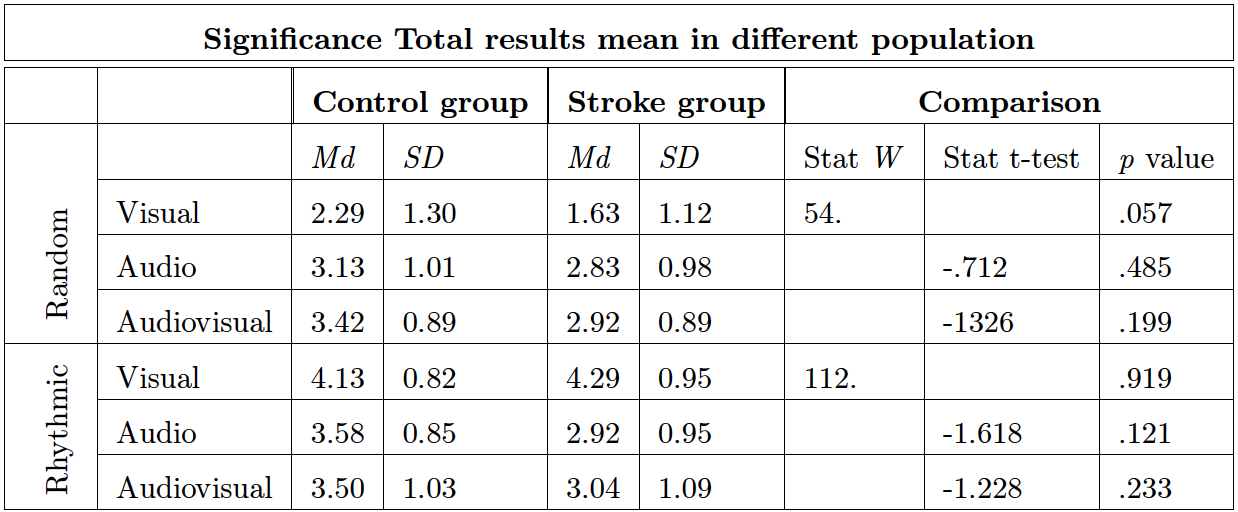
\includegraphics[width=0.70\textwidth]{significance_tables/tot_mean_pop.png}
    \caption{Significance of the results of all behavioral questions, comparing different population groups, using Wilcoxon Signed-Rank Test (\textit{W}) or Paired Samples t-Test (\textit{t}); \textit{M} = mean; \textit{SD} = standard deviation}
    \label{fig: significance_total_mean_pop} 
\end{figure} 

\clearpage
\subsection*{Results related to correlations}
\begin{figure}[H]
    \centering
    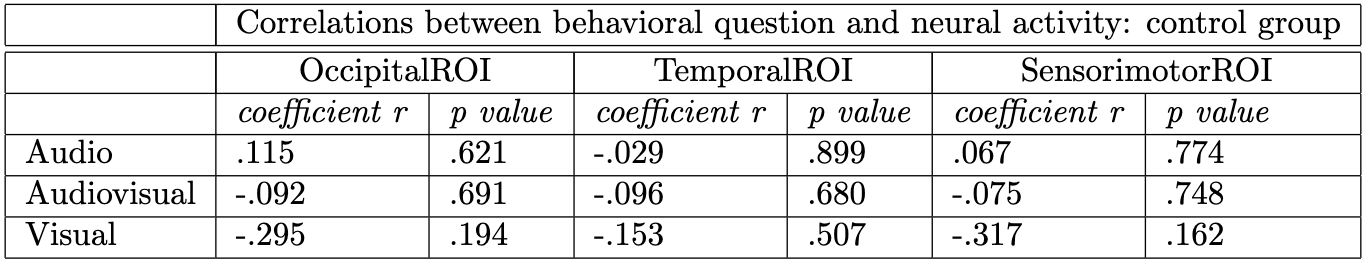
\includegraphics[width=0.75\textwidth]{scatter_plots/correlation_q2_control.png}
    \caption{Correlation values: Spearman correlation coefficient \textit{r} and \textit{p} value}
    \label{fig: correlation values q2: control} 
\end{figure}

\begin{figure}[H]
    \centering
    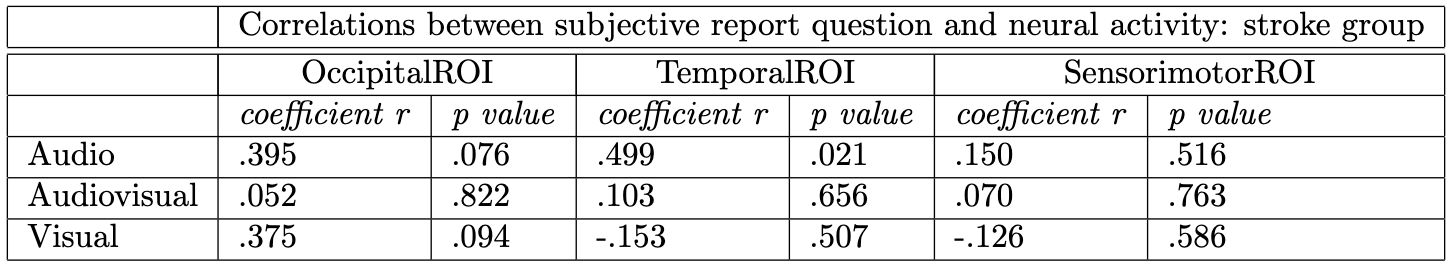
\includegraphics[width=0.75\textwidth]{scatter_plots/correlation_q2_stroke.png}
    \caption{Correlation values: Pearson correlation coefficient \textit{r} and \textit{p} value}
    \label{fig: correlation values q2: stroke} 
\end{figure}

\begin{figure}[H]
    \centering
    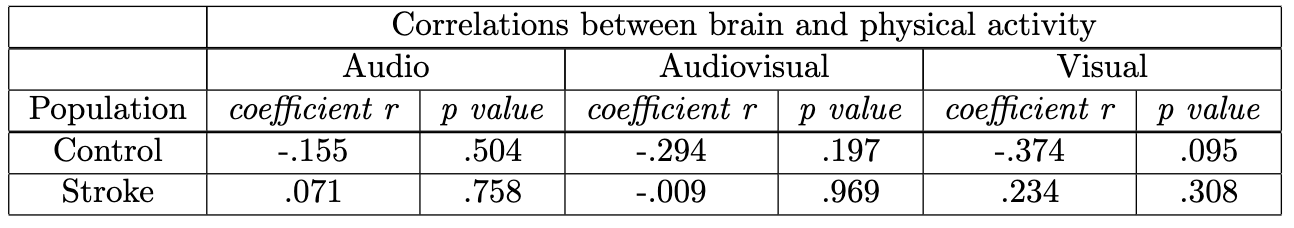
\includegraphics[width=0.75\textwidth]{significance_tables/correlation_activeq_.png}
    \caption{Correlation values: Spearman's correlation coefficient \textit{r} and \textit{p} value}
    \label{fig: significance correlation activeq} 
\end{figure}

\newpage
\thispagestyle{empty}
% \clearpage
% \chapter*{Results}
% \subsection*{Topographies}
% \begin{figure}[htbp]
%     \centering
%     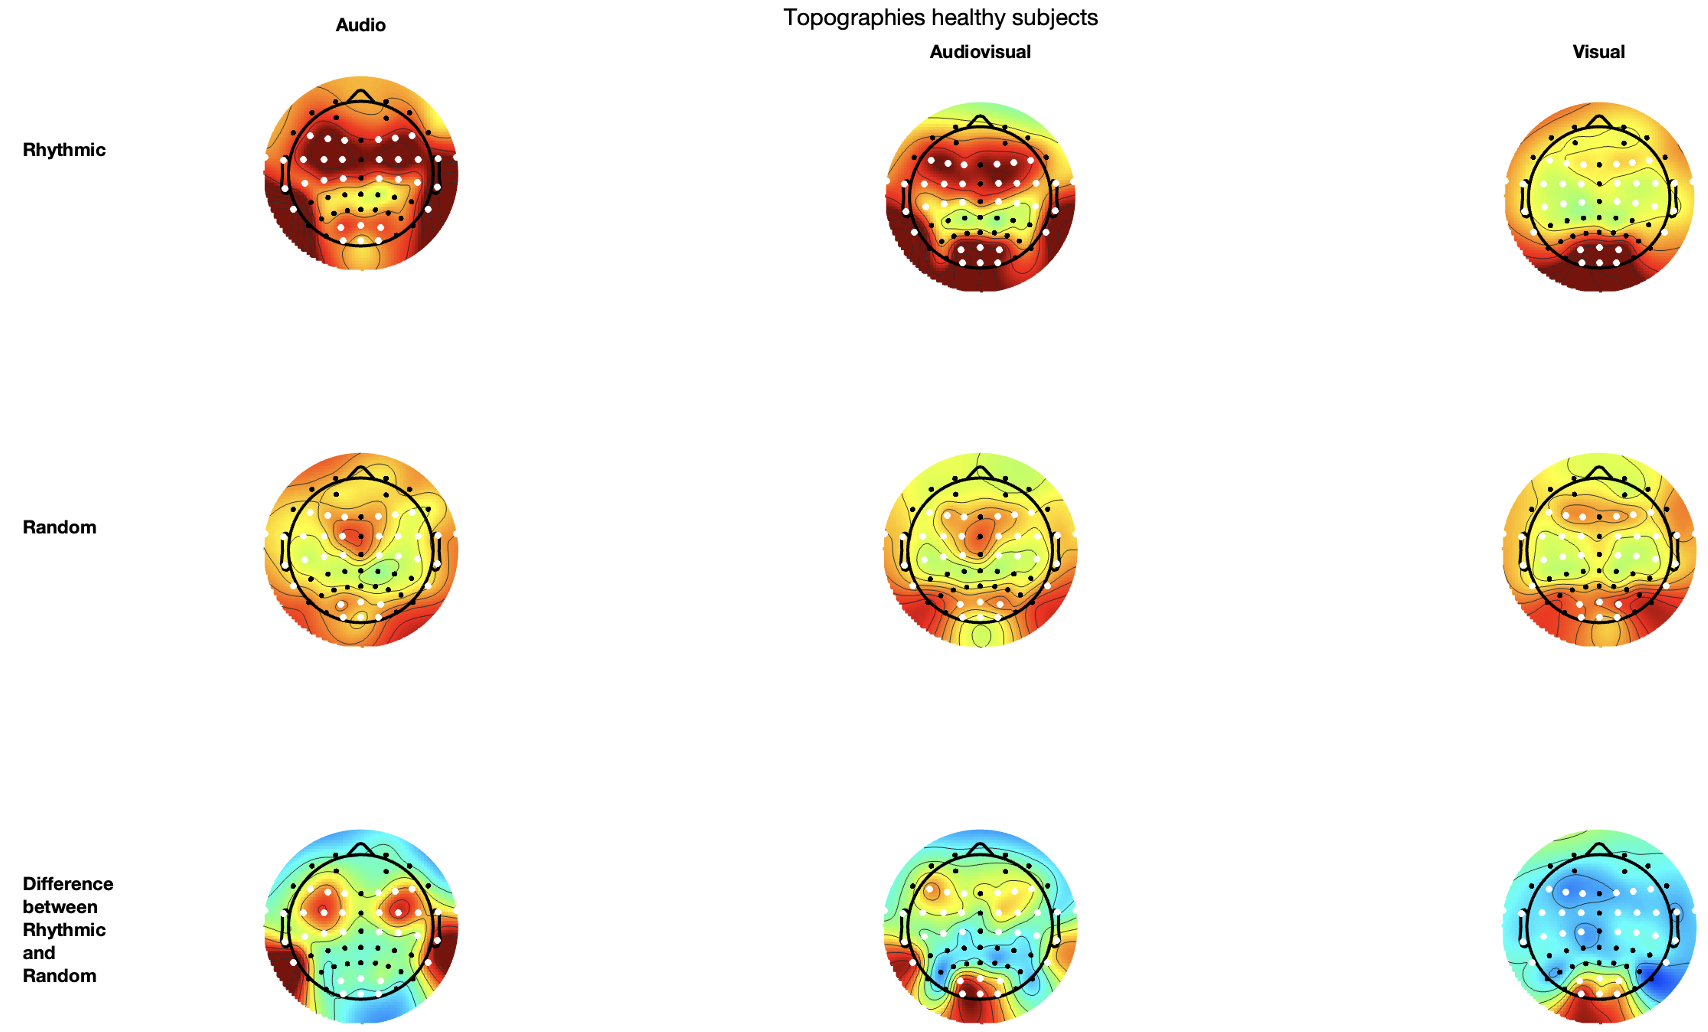
\includegraphics[width=0.95\textwidth]{healthy_images/topo.png}
%     \caption{Topographies related to the activity in the control group}
%     \label{fig: topographies control group}
% \end{figure}
% \begin{figure}[htbp]
%     \centering
%     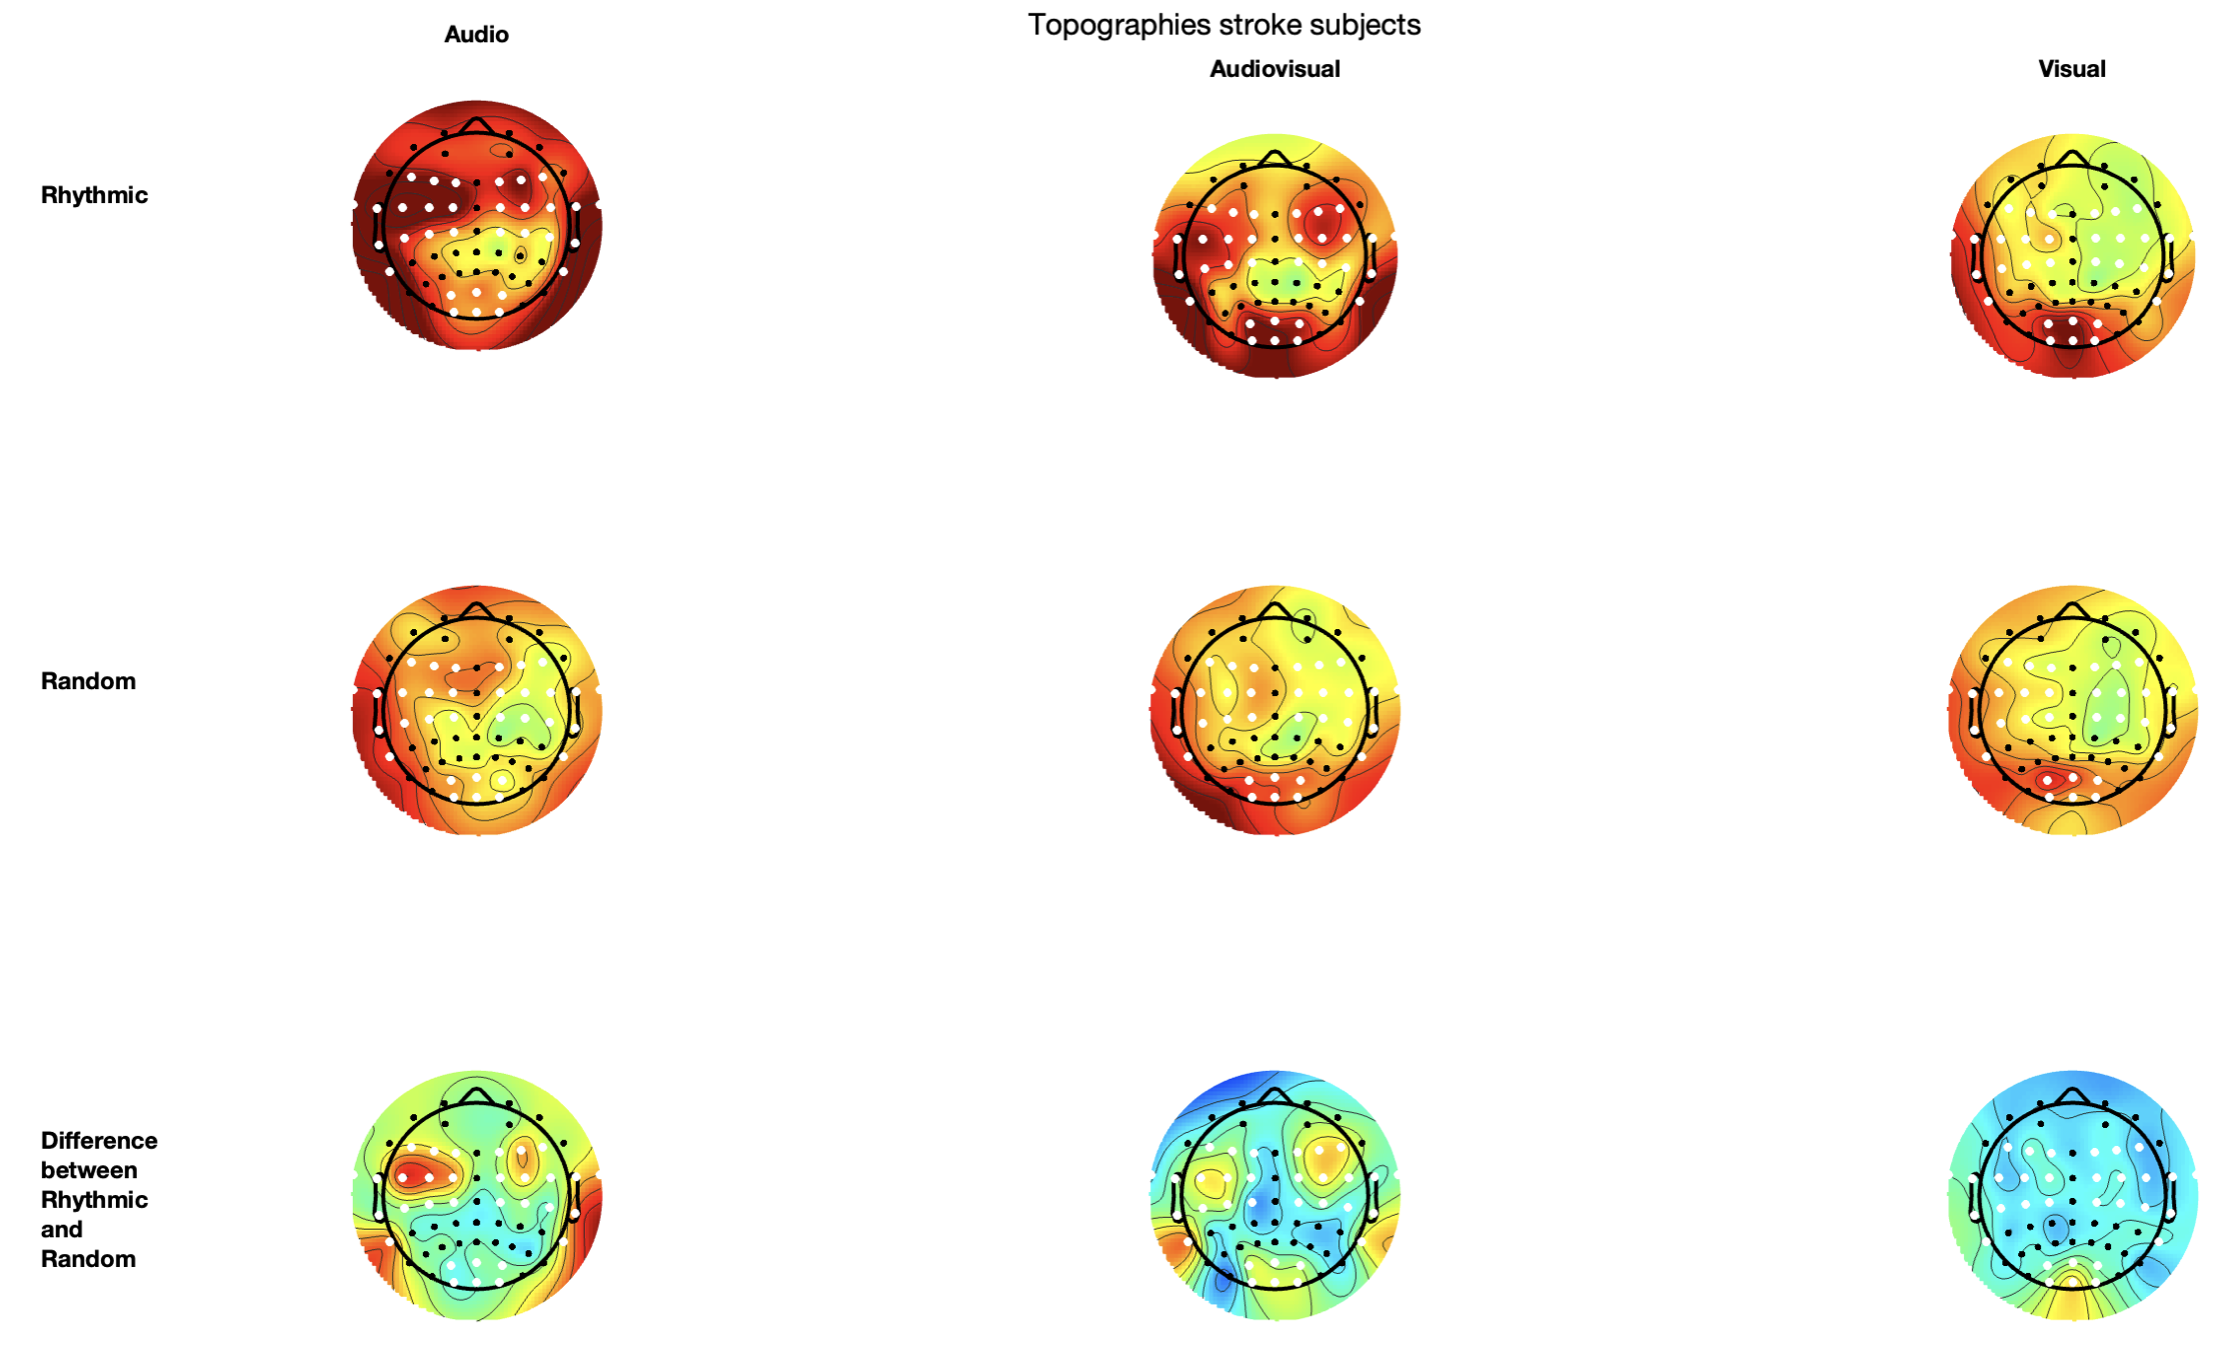
\includegraphics[width=0.85\textwidth]{stroke_images/topographies.png}
%     \caption{Topographies related to the activity in stroke population}
%     \label{fig: topographies stroke group}
% \end{figure}
% \begin{figure}[htbp]
%     \centering
%     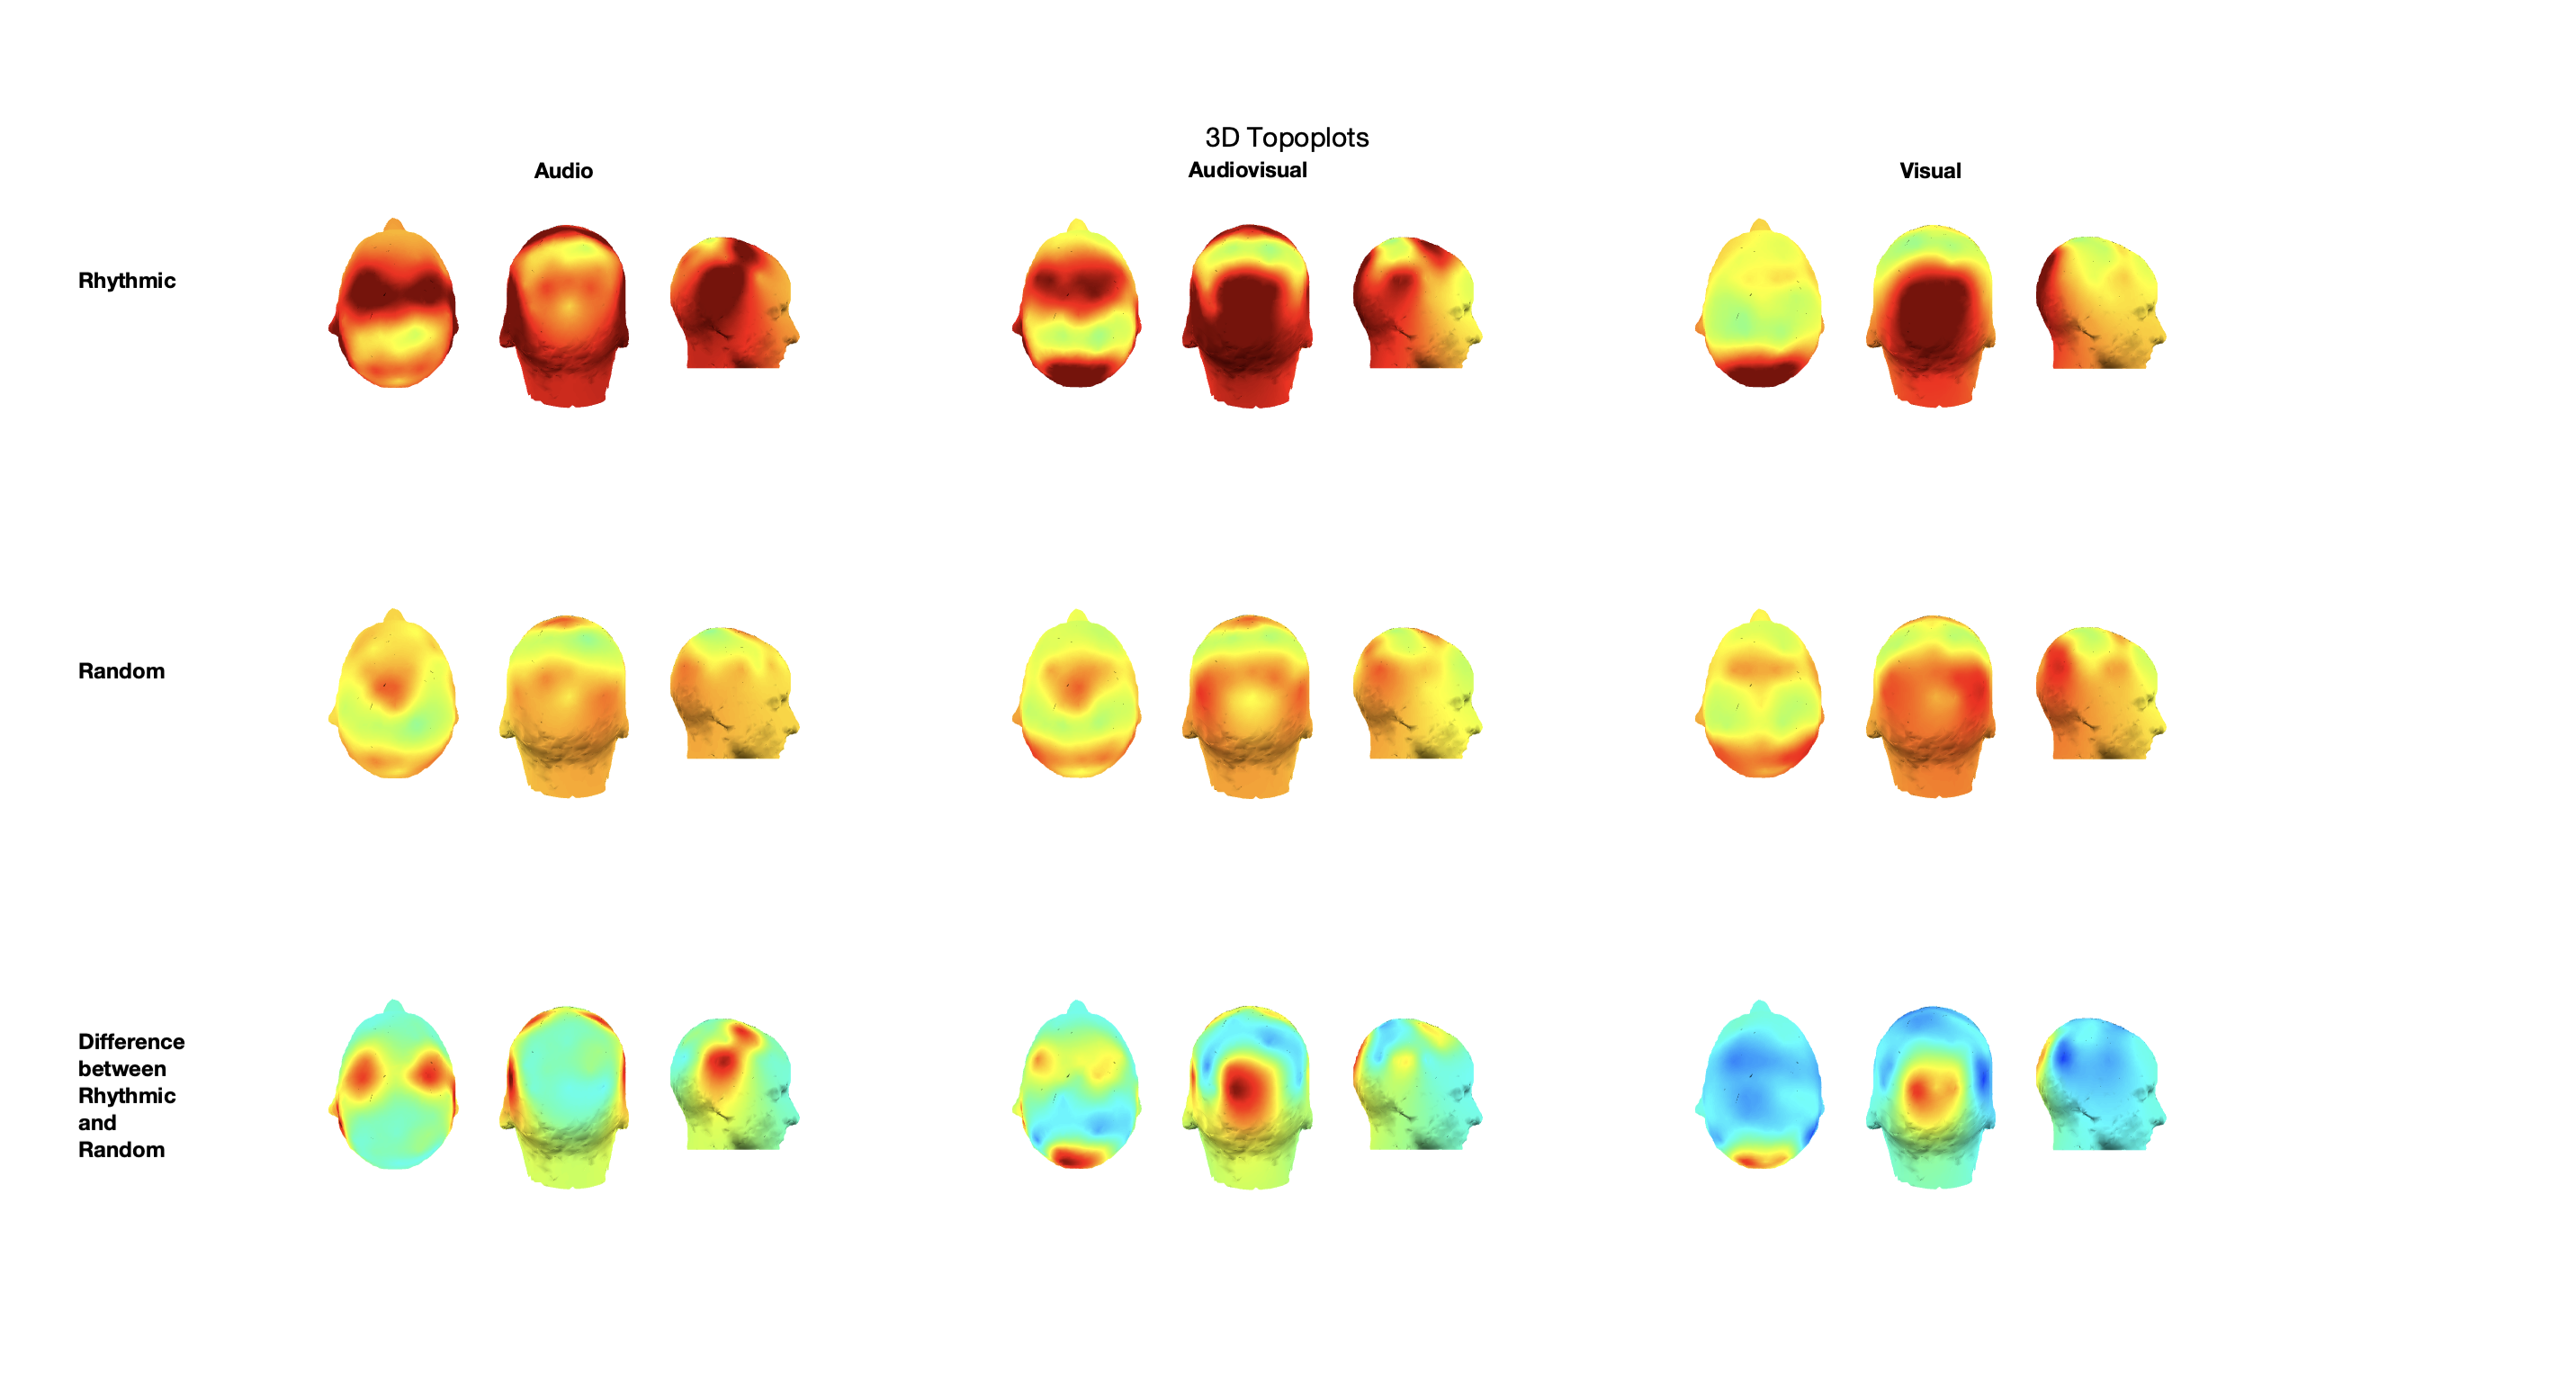
\includegraphics[width=0.85\textwidth]{healthy_images/3d_topo.png}
%     \caption{3D topographies related to the activity in the control group}
%     \label{fig: 3D topographies control group}   
% \end{figure} 
% \begin{figure}[htbp]
%     \centering
%     \includegraphics[width=0.85\textwidth]{stroke_images/3d_topographies.png}
%     \caption{3D topographies related to the activity in stroke population}
%     \label{fig: 3D topographies stroke group}   
% \end{figure} 
% \clearpage
